\documentclass[a4paper,10pt]{article}

\usepackage[boxruled,vlined,english]{algorithm2e}
\usepackage[francais,english]{babel}
\usepackage[utf8x]{inputenc}
\usepackage[T1]{fontenc}
\usepackage{graphicx}
\usepackage{hyperref}
\usepackage{latexsym}
\usepackage{setspace}
\usepackage{amsmath}
\usepackage{amssymb}
\usepackage{bookman}
\usepackage{amsthm}
\usepackage{amscd}
\usepackage{color}
\usepackage{calc}

\setlength{\voffset}{-3.75cm}
\setlength{\hoffset}{-2.6cm}
\setlength{\oddsidemargin}{2.25cm}
\setlength{\topmargin}{4cm}
\setlength{\headheight}{0in}
\setlength{\headsep}{0in}
\setlength{\topskip}{0in}
\setlength{\parindent}{0cm}
\setlength{\parskip}{1ex plus0.4ex minus0.2ex}
\setlength{\textwidth}{17.25cm}
\setlength{\textheight}{23cm}
\renewcommand{\baselinestretch}{1.5}
\flushbottom
\setcounter{page}{1}
\setcounter{tocdepth}{2}

\SetKw{Edb}{Side effect}
\SetKw{Et}{and}
\SetKw{Ou}{or}
\SetKw{De}{from}
\SetKw{A}{to}
\SetKw{Par}{by}
\SetKwBlock{Debut}{Begin}{End}
\SetKwIF{Si}{SinonSi}{Sinon}{If}{then}{Else if}{Else}{EndIf}
\SetKwFor{Pour}{For}{do}{EndFor}
\SetKwFor{PourTout}{For all}{do}{EndFor}
\SetKwFor{TantQue}{While}{do}{EndWhile}
\SetKw{Retour}{Return}

\newcommand{\guill}[1]{“#1”}
\newcommand{\bigO}[1]{\mathcal O\left( #1 \right)}
\newcommand{\bigOmega}[1]{\Omega\left( #1 \right)}
\newcommand{\bigTheta}[1]{\Theta\left( #1 \right)}




% ??? Faire une Titlepage un peu plus jolie...
\title{ \Large Internship report \\ \LARGE Computational analysis of jazz chord sequences}

\author{\normalsize Romain \textsc{Versaevel}, M1 Informatique Fondamentale, ENS de Lyon\\
\normalsize Tutored by David \textsc{Meredith}, Associate professor at Aalborg University,\\
\normalsize leader of the Music Informatics and Cognition group\\}

\date{\today}

\begin{document}

\maketitle

\begin{abstract}
\noindent
I report here the results of my work at Aalborg University during the summer 2015. My main task was to provide an analysis of a dataset of chord sequences of 30 jazz songs. The ultimate goal is to understand jazz better thanks to this kind of investigations.

\noindent
The analysis I propose studies the compression of the dataset, with two algorithms: the LZ77 compression algorithm and an algorithm computing \emph{diagonal patterns}. Their performances in terms of \emph{compression factors} were improved by introducing compression with loss through the use of \emph{similarity measures} between chords. The obtained analysis is successful; it validates my methods and shows room for further research; its main suggests that the structure of jazz chord sequences structure should rather be seen as a whole than linearly.

\noindent
The algorithms, their results, as well as a short introduction to computer music can be found in the report.
\end{abstract}

\newpage
\tableofcontents
\newpage


\section{Introduction}

This report presents the three-month internship I did as part of my Master 1 of Computer Sciences at ENS Lyon. This internship took place at Aalborg University, Denmark, from May 25th, 2015 to August 14th, in the Department of Architecture, Design and Media Technology. I was supervised by Prof. David Meredith, who specializes in computer music.

During this internship I mainly worked on computational music analysis, and more specifically on the analysis of a dataset of chord sequences from popular jazz songs. And extract of this dataset (presented in section \ref{motivation}) gathered by the Sony CSL research laboratory was provided to Aalborg University, in order to be studied.

The report has three main sections.
The first one is an introduction to the research field, \emph{computer music}.
The second section describes my work on the jazz chords dataset, consisting in two different ways of compressing it, and the obtained results.
Finally, the third section presents other related developements I started investigating, together with possible research directions.

An appendix with more details (additional definitions, examples of the algorithms execution, exhaustive numerical results\dots) can be found on \href{https://github.com/Rometach/aalborg/blob/master/Rapport/appendix.pdf}{the GitHub repository} I used.



\section{Computer music}

This section briefly introduces the area of computer music. The non-expert reader can find here a glimpse of the context and motivation of my work. I present first the general field, and then the more specific domain of computational music analysis.


\subsection{Short presentation and research areas}

The terms \emph{computer music} simply describe any activity that implies both music and computing tools.

Music and mathematics have been connected from origins. Links are numerous throughout history (see \cite{musicmaths} for example). The basis of western music was developed by the Pythagoreans in the 5th century BCE. The musical stave\footnote{~~In French: \emph{portée}.} was invented during the 12th century, five hundred years before Cartesian coordinate systems. The French composer Jean-Philippe Rameau used mathematical tools to theorise harmony in the 18th century, in \cite{rameau} for example. Modern composers such as Messiaen, Schönberg, or Xenakis\footnote{~~See for instance Xenakis, I. (1992). \emph{Formalized music: thought and mathematics in composition} (No. 6). Pendragon Press.} investigated new forms through mathematics. Sound is a physical vibration, and has mathematical properties; and western music is structured at every level by numbers. Hence, the birth and development of computer music naturally quickly followed the one of computers. The progress of computation offered new tools to musicology; simultaneously, the all-analogue world of audio became almost all-digital.

Computer music is therefore a young science (the first pieces composed with the help of computers appeared in the late 50s), based on a very ancient one. In computer sciences, it is related to computational linguistics; it can be close to cognitive sciences and often uses techniques from machine learning.

Its research areas are numerous and diversified. One can deal with audio data (recordings, live performance\dots) or symbolic one (MIDI scores\dots); one can study existing pieces or aim at producing new ones; one can improve the laypersons' or the professional musicians' experience. Here is a non-exhaustive list of research areas being part of computer music:

\begin{tabular}{rl}
$\triangleright$ & automated composition or orchestration; \\
$\triangleright$ & automated live improvisation; \\
$\triangleright$ & computational music analysis; \\
$\triangleright$ & music representation; \\
$\triangleright$ & signal processing\dots\\
\end{tabular}


\subsection{Computational music analysis}

Why analyse music with computers? As stated above, computers provide researchers with brand new ways of studying music. My analysis, for example, requires too many computations for a human being, and on the other hand no peculiar musical skills. And what kind of \emph{analysis} can computers achieve? Anything that can help the work of musicologists will be called an analysis; the most common ways to do so are pattern discovery (as in the analysis that follows) and segmentation into meaningful units.

An analysis can be of audio material or of symbolic representation (or both); its goal can be to acquire knowledge or the ability to create new pieces (or both). The analysis I give here focuses only on symbolic data and its purpose is rather a learning one.

At the beginning of my internship, my work was mainly bibliographical, in order to become more familiar with the diversity of existing techniques for computational music analysis. A reader who would like to do the same may want to read papers using probabilistic grammars (\cite{goldabdallah}), Markov chains and $n$-grams (\cite{markov1}, \cite{markov2}, \cite{markov3}), geometrical patterns (\cite{cosiatec}), or tries (prefix trees) (\cite{patminr}).


%\subsection{Several techniques}
%
%\subsubsection{Schenker}
%\subsubsection{http://webprojects.eecs.qmul.ac.uk/marcusp/papers/PearceWiggins2012.pdf}
%\subsubsection{http://axon.cs.byu.edu/~dan/673/papers/pachet.pdf}
%\subsubsection{http://citeseerx.ist.psu.edu/viewdoc/download?doi=10.1.1.3.5364&rep=rep1&type=pdf}
%\subsubsection{COSIATEC}
%\subsubsection{PatMinr}


\newpage
\section{Analysing jazz chord sequences}

In this section, after a presentation of the data motivating this project, jazz lead sheets, I introduce the main tools I used, namely compression algorithms chord similarity measures. Finally I present and discuss my results.

\subsection{Motivation}
\label{motivation}

The project was mainly motivated by an extract of a dataset of jazz lead sheets. This dataset was provided by \href{http://www.csl.sony.fr/music.php}{Sony CSL}, a research laboratory located in Paris of Sony Corporation, one of the world leading companies in audio technology. Data are an important issue in computer music, because most musical materials are not digitized yet, and databases are hard to gather. My task was to provide an analysis of this dataset.

Before going into more details, I have to introduce basic musical definitions. I try here to give enough explanations for anyone to understand what I will deal with, but also clues for a more interested or knowledgeable reader who would like to get a glimpse of mathematical models of music.

In jazz music, songs are displayed in the form of \emph{lead sheets}, scores giving the base melody with extra indications of chords. An extract of a lead sheet for \emph{What a wonderful world} by Louis Armstrong (1967) illustrates this in Figure \ref{waww}; the sung melody is written on a stave and the chords are visible in handwritten font.

\begin{figure}[h!]
\centering
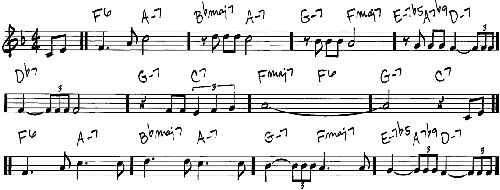
\includegraphics[width=10cm]{images/waww.jpg}
\caption{Lead sheet with the beginning of Louis Armstrong's \emph{What a wonderful world}.\label{waww}}
\end{figure}

A \emph{chord} is a set of at least three notes; in the jazz context, they are given as an indication of the current atmosphere of the piece, and musicians can improvise the accompaniment of the melody with the notes of the chord. Chords are represented\footnote{~~There are several ways of representing chords; this representation, sometimes called the \emph{tabular notation}, is the most common in popular music (jazz, pop, rock\dots). However, superposed notes on a classical music stave would also represent a chord.} 
by a letter\footnote{~~The French equivalent is to give names to notes, from \emph{do} ($C$) to \emph{si} ($B$).} from $A$ to $G$ 
with a possible \emph{accidental} ($\#$ for \emph{sharp}, $\flat$ for \emph{flat}, or nothing), representing the \emph{root note}, and a textual information giving the other notes relative to the root note. For example, if we consider the $C\#m7$ chord (\guill{$C$ sharp minor seventh}), the notes will be the root note, $C\#$, its \emph{minor third}, $E$, its \emph{fifth}, $G\#$ and its \emph{minor seventh}, $B$. There are 313 different such textual informations in the Sony dataset\footnote{~~With the model of section \ref{chordmodel}, one could theoretically form 2037 different chords for a given root note (number of subsets of size at least 2 of a set of size 11); the actually used chords correspond to the \guill{harmonious} combinations, which is a subjective notion and thus depends on the music genre.}.

The dataset I worked on contains the lead sheets of 30 jazz pieces by famous artists like Louis Armstrong, Billie Holiday or Charlie Parker. It is an extract of a larger set gathered by Sony CSL. I used only the files describing the chord sequences\footnote{~~Other files described the melodies (with pitch, onset and duration).}. They were written in plain text format, and contained in all 1469 chords, given in the previous representation. The sequence below shows an example of how this data was encoded:

\begin{equation*}
\text{\textbf{A Child Is Born:} } B\flat M7;~E\flat m;~B\flat M7;~E\flat m6;~B\flat M9;~E\flat m;~A~halfdim7;~D 7\#9\dots
\end{equation*}

So, the motivation for my work was to provide an analysis of this data. The purpose of such an analysis is to gain knowledge about jazz and chord sequences, understanding it better, and also in a second time to use this knowledge to be able to compose similar music that would fit in the corpus. Since I wanted an analysis of the entire data rather than analyses of each piece, I used as an input for the algorithms described in \ref{algos} a concatenation of the 30 songs: the sequence of all the 1469 chords.



\subsection{Compression algorithms}
\label{algos}

The words \guill{analysis} and \guill{compression} will be used here with very close meanings. Indeed, compressing a piece means exhibiting its structure and separating the essential from the redundant. In other words, the analysis I did consisted in looking at how jazz chord sequences can be compressed, and interpreting the results of compression processes as new knowledge on jazz music. Hence, my analysis of the jazz lead sheets dataset will be described in terms of compression, and evaluated as such.

There are two complementary ways to approach computational music analysis\footnote{~~They are of course also relevant in a wider context.}. 
One sees a piece as a linear sequence of notes (or chords, etc.), as the listener does: she can remember everything she heard but has no way to know what is coming until she actually hears it. The other approach views the piece from above, completely. In terms of data structures, the former considers the piece as a linked list and the latter as an array. \guill{Linear} analyses use for example Markov models and Shannon's entropy; \guill{global} analyses use for likely formal grammars and Kolmogorov's complexity.

The compression method I use simply describes a sequence of chords through the patterns (repeated sub-sequences) it contains, thus removing the redundancy. I designed, implemented and tested algorithms for both approaches (linear and global), in order to be able to compare them. For the former, I used the classical algorithm known as LZ77; for the latter, a \guill{diagonal pattern decomposition}. They are presented in this order.


\subsubsection{Lempel-Ziv 77 (LZ77)}

The first algorithm (for the linear approach) is LZ77. It was designed by A. Lempel and J. Ziv in 1977, introduced in \cite{lempelziv}, and is a very popular compressing algorithm. I chose it because it is simple and efficient (most dictionary coders are based on it).

It takes as an input a list (so, a stream) of data and produces as an output a list of triples of the form $(a,b,D)$ meaning: \guill{go back $a$ times, copy the next $b$ data, and add $D$}. In the original algorithm, restrained buffer and preview size are given as parameters; however, I decided to let them be unbounded in order to focus on the best possible results. The obtained algorithm is written in Algorithm \ref{algolz77}, and a complete illustrative example of an execution is given in the appendix.

\begin{algorithm}
\setstretch{1.5}
\caption{LZ77 \label{algolz77}}
\SetKwData{iii}{i} \SetKwData{jjj}{j} \SetKwData{III}{$\texttt{I}$} \SetKwData{pref}{$\pi$} \SetKwData{aaa}{a} \SetKwData{bbb}{b} \SetKwData{buffer}{$\texttt{buffer}$} \SetKwData{LLL}{$\texttt{L}$}
\SetKwFunction{push}{push} \SetKwFunction{pop}{pop} \SetKwFunction{front}{front} \SetKwFunction{size}{size}

\KwIn{Queue of Chords $\III=(C_1, \dots, C_n)$.}
\KwOut{Queue of triples $\LLL=(a_j,b_j,C_{i_j})_j$.}

\Debut {
	\buffer $\leftarrow$ empty queue 

	\TantQue{\III is not empty} {
		\pref $\leftarrow$ longest prefix of \III in $(\buffer\cdot\III)$, beginning in \buffer

		\aaa $\leftarrow$ $\size(\buffer)$ $-$ (beginning index of \pref (in \buffer)) ($0$ if none)

		\bbb $\leftarrow$ length of \pref ($0$ if none)

		\Pour{\jjj \De $1$ \A \bbb} {
			$\buffer.\push(\front(\III))$

			$\III.\pop()$
		}
		$\LLL.\push(\aaa,\bbb,\front(\III))$

		$\buffer.\push(\front(\III))$

		$\III.\pop()$
	}
	\Retour \LLL
}
\end{algorithm}

With a computation of the longest prefix in $\bigO{|\texttt{I}|^2}$, the overall complexity is $\bigO{|\texttt{I}|^3}$. There are more accurate evaluations of this complexity, discussed among other in \cite{lempelziv}, though not of much interest here. Knowing that the complexity is polynomial and that the implementation runs fast is enough.


\subsubsection{Diagonal pattern decomposition}
\label{compressiondiagonal}

The second algorithm (for the global approach) uses \emph{diagonal patterns}. The best way to understand this notion is to visualise it. For a given piece, we write the chord sequence both vertically and horizontally. We can then consider a matrix whose cell $(i,j)$ will correspond to the $i$th and $j$th chords of the input sequence. Let us draw this cell in white if these chords are identical, and in black if they are different. We get a binary matrix by which we can see the diagonal patterns, which are diagonal sequences of white cells. They correspond to sequences of chords that appear (at least) twice in the input piece, on two different positions. Figure \ref{diagonals} shows such a matrix (for an extract from \emph{Giant Steps}, by John Coltrane).

\begin{figure}[h]
\centering
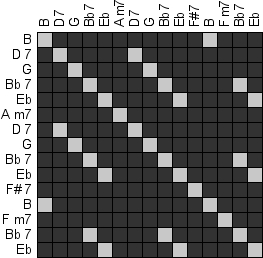
\includegraphics[width=6cm]{images/diagonals1.jpg}\hspace{1cm}
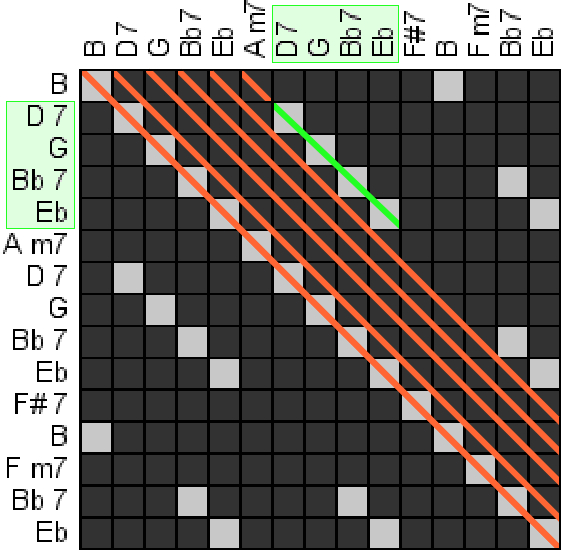
\includegraphics[width=6cm]{images/diagonals2.jpg}
\caption{A binary matrix and the diagonal search for patterns.\label{diagonals}}
\end{figure}

The \emph{patterns} selected by the algorithm precisely are maximal diagonal sequences, along with their occurrences (positions where they occur). \emph{Maximal} means that we consider only sequences having an occurrence that cannot be extended. Figure \ref{diagonals} shows the diagonal search for patterns and the maximal pattern $D7;G;B\flat 7;E\flat$. $D7;G$ is not maximal: every times it occurs it can be extended in the end. On the contrary, $B\flat 7;E\flat$, which is included in $D7;G;B\flat 7;E\flat$, is also a maximal pattern, occurring in the very end. In the piece of Figure \ref{diagonals}, the diagonal patterns are (by increasing size):

\begin{tabular}{rl}
$\triangleright$ & $B$, at positions 0 and 11; \\
$\triangleright$ & $B\flat 7;E\flat$, at positions 3, 8 and 13; \\
$\triangleright$ & $D7;G;B\flat 7;E\flat$, at positions 1 and 6.\\
\end{tabular}

Once the list of patterns is established, the next step is to select a subset of these patterns which is sufficient to describe the whole piece. It can happen, like in the current example, that it not possible to completely cover the input piece with the diagonal patterns. To tackle this issue, we add a \guill{pattern} for each single chord appearing in the piece (here: $B$ at positions 0 and 11, $D7$ at position 1, $G$ at position 2\dots). The selected subset should be as \guill{light} as possible, the \emph{weight} of a pattern being the sum of its length and of its number of occurrences. This problem is a \emph{weighted set cover}, which is NP-complete\footnote{~~For more explanations on the set cover problem, see \cite{karpNP} or \cite{cormen}.}. So I implemented two heuristics, and the lighter results of the two is selected. Briefly, they are both greedy algorithms; one aggregates patterns until covering the whole piece and the other removes as many patterns as possible from the exhaustive list. Their pseudo-codes are given in the appendix.

The complexity of the whole algorithm is $\bigO{|\texttt{I}|^5}$~\footnote{~~See appendix for a brief analysis.}. This is quite high. In practice, the number of maximal patterns (which is $\bigO{|\texttt{I}|^2}$ in the worst case) seems to be the most determining factor for the running time. On my complete database (approximately 1500 chords), the execution takes between a few seconds and several minutes.


\subsection{Similarity measures for chords}

This section introduces the concept of chord similarity measures, and how I used them to improve the algorithms from previous section. Specific similarity measures have been developed for chords, to quantify formally their audible differences. I define here a mathematical model of chords, and then the state-of-the-art measures I used. Finally I present their incorporation into the algorithms and its consequences.

\subsubsection{A mathematical model of chords}
\label{chordmodel}

There are only 12 possible root notes because two notes separated by an \emph{octave} (concretely, whose frequencies ratio is a power of two) sound the same, and are thus called the same: $C$ refers to low-pitched as well as to high-pitched sounds. The 12 notes correspond to a division of the octave into twelve equally spaced \emph{semitones}; this is called the \guill{well-tempered} scale. 
So, as shown in Figure \ref{keyboard}, the keyboard can be mapped to the cyclic group $\mathbb{Z}/12\mathbb{Z}$, and the notes to integers from $0$ to $11$\footnote{~~Usually, $C$ is mapped to 0; it has no importance here and I chose to map $A$ to 0 instead, which seemed simpler.}.

\begin{figure}[h!]
\centering
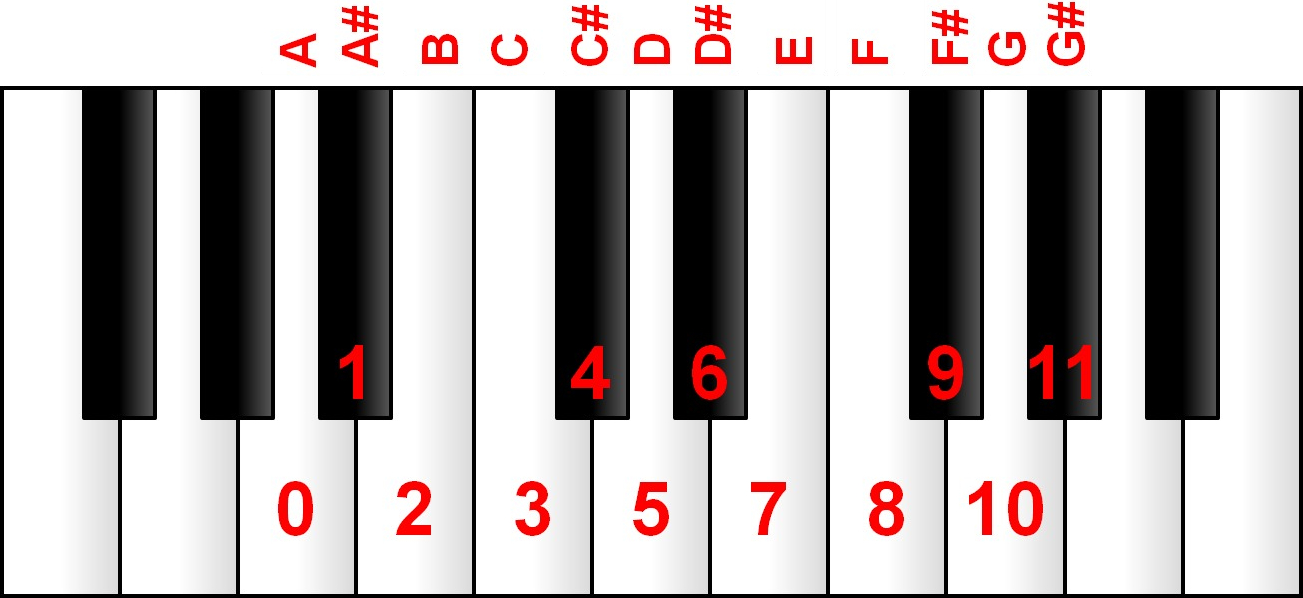
\includegraphics[width=7
cm]{images/keyboard2.jpg}
\caption{A keyboard with note names and their mapped values in $\mathbb{Z}/12\mathbb{Z}$.\label{keyboard}}
\end{figure}

Chords can then be seen as subsets of $\mathbb{Z}/12\mathbb{Z}$. For instance, the previously seen $C\#m7$ chord would be mapped to the set $\{4;7;11;2\}$~\footnote{~~The order can be important, but does not matter here.}. Moreover, the harmonic content in the chord name (here, \guill{$m7$}) can be seen as a vector and the root note (\guill{$C\#$}) as a starting point. Chords with same labels but different root notes are then the same by transposition: $C\#m7$ corresponds to $\{4;7;11;2\}$ and $D\#m7$ to $\{5;8;12;3\}=\{4;7;11;2\}+\{1;1;1;1\}$.

It is hence possible to define formal distances between chord. However, such a distance must be chosen carefully to be relevant. Canonical distances do not necessarily mirror what is heard. With the \guill{city block distance}) on chords of three notes, the chords $C=\{3;7;10\}$ and $Cm=\{3;6;10\}$ would be close since the difference is only of one semitone; but to the ear they sound very different, one being major and the other minor. Likewise, $C=\{3;7;10\}$ and $Bm=\{2;5;9\}$ would sound closer than they may look: they are \guill{inversions} of each other.


\subsubsection{List of used measures}

In all, I used 10 different measures (including equality), some of which are rather elementary, and some specifically developed for this field. Three take as an input the two chords to compare, $C_1$ and $C_2$, and return a boolean (\texttt{true} if and only if the chords are similar). All three define equivalence classes. They are:

\begin{itemize}
\itemsep0em 
\item[$\triangleright$] root note equivalence: \texttt{true} iff $C_1$ and $C_2$ have the same root note;
\item[$\triangleright$] transposition\footnote{~~The word \guill{transposition} in music correspond to the geometrical notion of \guill{translation}.} 
equivalence: \texttt{true} iff $C_1$ and $C_2$ have the same harmonic indication (but possibly different root notes);
\item[$\triangleright$] PCS-Prime equivalence (see \cite{forte}): \texttt{true} iff $C_1$ can be obtained from $C_2$ by a combination of inversions and transpositions.
\end{itemize}

The six other measures are distances\footnote{~~I use the word \guill{distance} to emphasize the difference with the first three measures; however all are not distances in a mathematical meaning.}: they take as an input two chords $C_1$ and $C_2$ and return a positive real number. As I will show in the next part, this value was needed only to determine if two chords are \guill{close} or \guill{different}, so I used them with a threshold as additional input parameter. The measure will then return \texttt{true} if and only if the distance between $C_1$ and $C_2$ is less than the threshold.

They are the F1-score (cardinality of the intersection divided by the sum of the cardinalities, multiplied by two); Eric Isaacson's similarity index, defined in \cite{isaacson}; David Lewin's measure, defined in \cite{lewin}; Robert Morris' measure, defined in \cite{morris}; John Rahn's measure, defined in \cite{rahn}; Richard Teitelbaum's measure, defined in \cite{teitelbaum}.

The definitions of all these measures can be found in the appendix. Here I will only present as an illustrative example Isaacson's similarity index. It is a relatively arbitrary choice since, as I will show in section \ref{resultsmeasures}, all these measures gave close results. Nevertheless, Isaacson's similarity index allows me to introduce the interesting notion of interval vector.

Given a set $S\subset\mathcal{P}([0,11])$, its associated \emph{interval vector} is a vector $IV(S)\in\mathbb{N}^6$ such that the $i$-th coordinate of $IV(S)$ is the number of pairs of elements in $S$ whose difference is $i$. In other words, we enumerate the intervals inside $S$: how many intervals of length $1$, of length $2$, etc. The interval vector is a histogram for these values. There are $6$ and not $12$ coordinates because these intervals are not oriented (modulo $12$, going from $1$ to $8$ is the same as going from $8$ to $12+1=13$, and the interval has then a length of $5$).

For example, for a major seventh chord, whose corresponding set is $\{0;4;7;10\}$, we have $1$ interval of length $2$ (between $0$ and $10$), $2$ of length $3$ ($4$ and $7$, $7$ and $10$), $1$ of length $4$ ($0$ and $4$), $1$ of length 5 ($0$ and $7$) and $1$ of length $6$ ($4$ and $10$). Hence $IV(\{0;4;7;10\})=(0,1,2,1,1,1)$. 

Isaacson's similarity index is defined as the \emph{standard deviation} function applied to the interval vectors. For chords $X$ and $Y$ with respective interval vectors $IV_X=(x_1,\dots,x_6)$ and $IV_Y=(y_1,\dots,y_6)$, let us denote by $D$ the difference vector $((y_1-x_1),\dots,(y_6-x_6))$ and $\bar{D}$ the mean of the $(y_i-x_i)$s. The measure is finally:

\begin{equation*}
\mathfrak{M}_{Isaacson}(X,Y) = \sqrt{\frac{1}{6}\left(\sum_{i=1}^6\left(D_i-\bar{D}\right)^2\right)}
\end{equation*}


\subsubsection{Improvement of the compression algorithms}

There exist \emph{lossy} and \emph{lossyless} compression algorithms. \emph{Lossyless} means that the decompression of the compression is equal to the original sequence, while it is not necessarily so with \emph{lossy} algorithms. The LZ77 algorithm and the diagonal patterns algorithm both perform a compression without loss. I transformed them into lossy algorithm; this allows better compression, i.\!e, smaller outputs. Again, the compression of jazz chord sequences is intended as an analysis. This is why I chose specific measures to musical analysis: improving the compression with meaningless measures would not be relevant.

The loss is introduced by replacing equality tests in the algorithms by similarity tests. In the LZ77 algorithm, equality tests occur when computing prefixes. Instead of the longest common prefix, the longest similar (for a given measure, up to a certain threshold if needed) prefix is selected. In the diagonal patterns algorithm, equality tests occurs when computing the binary matrix. Instead of drawing a cell of the matrix in white only if the two corresponding chords are equal, this will be done also if they are similar (for a given measure, up to a certain threshold if needed). The matrix has then more white cells, implying more and longer patterns. Figure \ref{loose} shows this transformation (with the F1-score and a threshold of $0.9$).

\begin{figure}
\centering
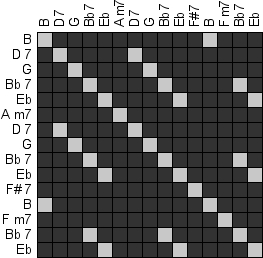
\includegraphics[width=5cm]{images/diagonals1.jpg}\hspace{1cm}
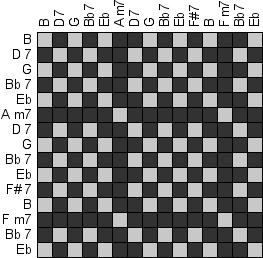
\includegraphics[width=5cm]{images/diagonals3.jpg}
\caption{Binary matrices for \emph{Giant Steps}, the second using a similarity measure (F1 score).\label{loose}}
\end{figure}

The compression processes are evaluated with their \emph{compression factor} and \emph{recovery factor}.

The \emph{compression factor} corresponds to the size of the input data divided by the size of the compressed data. It is expected to be as high as possible (and at least greater than $1$). I consider that the size of a chord is the same as the size of an integer. Indeed, they are $7\cdot4\cdot313=6573$ possible chords, so a chord can be described with $\lceil log_2(6573)\rceil = 13$ bits; and the integers dealt with are lesser than $1469$ (the total number of chords in the database), thus defined by $\lceil log_2(1469)\rceil = 11$ bits. Of course, this definition fits the data I used and a different one could be needed for a different dataset.

The \emph{recovery factor} is the ratio of chords in the decompression of the compression which are equal to the corresponding chords in the input piece. It is thus a real number between $0$ and $1$, that we will expect to be as close to $1$ as possible. This definition is rather sensitive. Indeed, the loss is introduced by the similarity measures: input chords are replaced during the compression process only by similar ones. The only other way to define the recovery factor would be to use precisely the similarity measure (\guill{the two corresponding chords are different by at most $t$ according to the measure}), however, in my eyes, not having an external evaluation would mean having too much faith in the measures. Moreover, while one understands well what it is to be equal or different, it is not clear what a difference of $t$ for a given precisely means.

So a decompression algorithm is needed to compute the recovery factor. It is very simple for the LZ77 algorithm. For the diagonal patterns algorithm, the covering patterns are sorted by increasing number of occurrences\footnote{~~This sorting criteria has been chosen empirically, because it led to the best recovery factors. Yet, is not clear why it should be better.} and are copied in this order (so, a position that is covered by several patterns is rewritten several times, and only the last written chord, coming from the pattern with most occurrences, will be kept). A pre-treatment is done on the patterns in order to maximize the recovery factor. Indeed, a pattern occurring \emph{similarly} several times can correspond to several different exact sequences, and the recovery factor will depend on the choice of the sequence (which does not impact the compression factor) representing the pattern. The pre-treatment simply consists in computing for every pattern what positions of the reconstruction depend on it, and choose among the possible sequences the one that implies a minimum loss\footnote{~~This greedy algorithm, knowing the decompression scheme, finds obviously the optimal configuration of this problem.}.



\subsection{Results}

The two algorithms have been run on the dataset of 1469 chords with all the measures and several thresholds. 
This section presents the results obtained by comparing the compression and recovery factors obtained by these compression processes. I focus here on their interpretation; more exhaustive numerical results can be found in the appendix. First the different measures are compared, and then the two algorithms.

\subsubsection*{Comparison between measures}

\label{resultsmeasures}
The 10 different measures I used resulted in different compression results. For different measures, binary matrices look differently; recovery and compression factors as functions of the thresholds look differently (as can be seen in the appendix). However, surprisingly, there is a correlation between these two factors, independent from the measure used, as can be seen in Figure \ref{rfc}, where . So, as one would have expected, there is a trade-off between the compression and the recovery factors: the better the compression, the higher the loss. Also, this feature validates the use of the F1-score, which in contrary to other measures was not designed specifically for music analysis, in this field.

\begin{figure}[h]
\centering
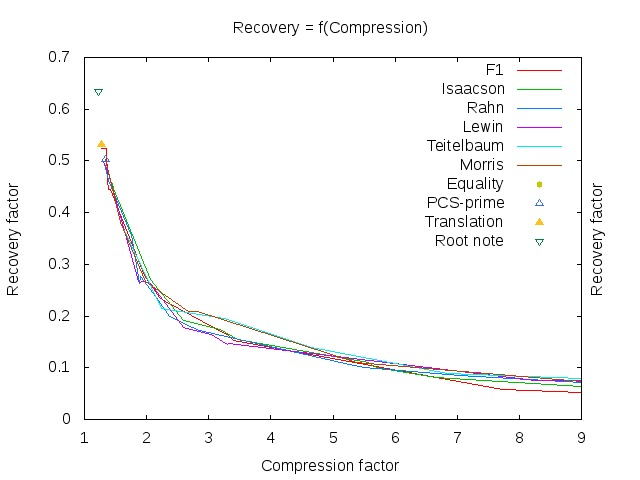
\includegraphics[width=7cm]{images/RfC77.jpg}\hspace{0.5cm}
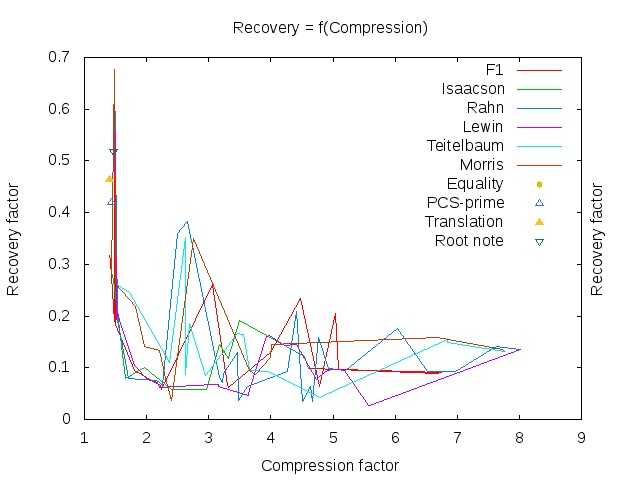
\includegraphics[width=7cm]{images/RfCDiag.jpg}
\caption{Link between recovery and compression factors (left: LZ77, right: diagonal patterns).\label{rfc}}
\end{figure}

In the case of the LZ77 algorithm, the results are really the same. Curves in Figure \ref{rfc} (left) have very close shapes. As for the diagonal patterns algorithm, some measures are \guill{leading} around several values of compression factors. But it is hard to determine if it comes from the irregularities of the algorithm or really originates from some kind of superiority. Roughly, leading measures are Teitelbaum's for compression factors between 1.5 and 2.5, Morris' between 2.5 and 3.5, Isaacson's similarity index between 3.5 and 4, the F1-score between 4 and 4.5, and again Morris' above 4.5.

As mentioned above, I use the recovery factor in order to benefit from an evaluation instrument that is exterior to the measures. Nevertheless, differences between them appear if we are confident in their ability to reflect musical closeness between chords. Indeed, in the case of the diagonal patterns algorithm, the best compression factors are not obtained for the same thresholds. All lead to highest compressions for medium thresholds, except for Isaacson's similarity index, shown in Figure \ref{isaacson}: the compression factor is almost an increasing function of the lossiness. This could be fortuitous, or mean that this precise measure is particularly adapted to the analysis of jazz chords. The best way to find out the truth would be to have the opinion of a skilled musician, who for instance would listen to the original piece and the decompression of the compression.

\begin{figure}[h]
\centering
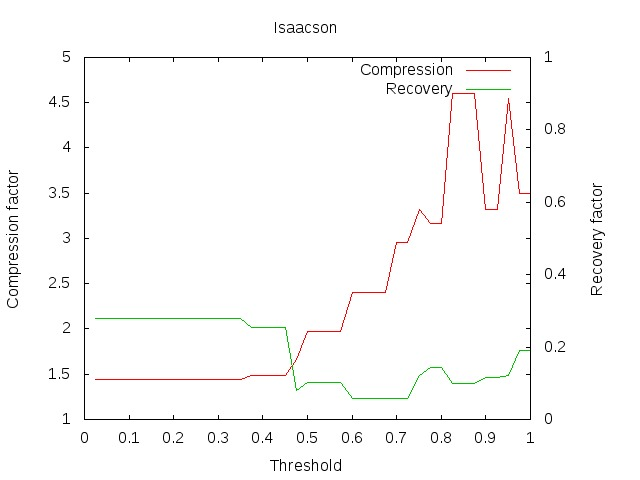
\includegraphics[width=7cm]{images/IsaacsonDiag.jpg}
\caption{Diagonal compression with Isaacson's measure.\label{isaacson}}
\end{figure}

\subsubsection*{The relevance of similarity measures}

The measures with no thresholds result in relatively low compression factors (and high recovery factors). The lossiless version of the LZ77 algorithm does not even compress: the compression factor is $0.931258<1$. The gain provided by the use of similarity measures becomes obvious with the ones using thresholds. They make possible a wide range of compression factors. 

The fact that \guill{loosening} the chord sequence actually improves the compression process brings to light the existence of a hidden structure of the pieces. It reveals that under an irregular surface there is a more simple shape. Using similarity measures smooths the surface and simplifies the analysis.


\subsubsection*{Comparison between algorithms}

The LZ77 algorithm produces much higher compression factors than the diagonal patterns algorithm. This is not surprising, as for an input size $|\texttt{I}|$, the shortest possible output of LZ77 is of constant length 2: $(0,0,\texttt{I}[1]),(1,|\texttt{I}|-2,C)$. For the diagonal patterns algorithm, the shortest possible output is of length $\sqrt{|\texttt{I}|}$: one pattern of length $\sqrt{|\texttt{I}|}$ occurring $\sqrt{|\texttt{I}|}$ times\footnote{~~The optimal compression is obviously composed of a single pattern; if it is of length $|\pi|$ it has to occur $\frac{|\texttt{I}|}{|\pi|}$ times, and its weight is then $|\pi|+\frac{|\texttt{I}|}{|\pi|}$, with a minimum for $|\pi|=\sqrt{|\texttt{I}|}$.}; 
and none of the implemented algorithms for the set cover problem would choose this configuration if all the chords of the input are similar.

The difference between the algorithms in terms of achieved compression factors is thus not very relevant. However, it is interesting to note that, for the measures without thresholds, the diagonal patterns algorithm obtains better compression factors (and lower recovery factors) than LZ77. For instance, when using the root note equivalence, the compression factor of LZ77 is 1.22421, while it gets to 1.46531 with the diagonal patterns algorithm (full results can be seen in the appendix).

Furthermore, one observes in Figure \ref{rfc} that the results of the diagonal patterns algorithm are a lot more \guill{chaotic} than the results of the LZ77 algorithm. Those are very regular: the compression factor is almost always a decreasing function (and the recovery factor an increasing function) of the similarity, represented by the threshold. One reason for the irregularities in the diagonal patterns algorithm is obviously the approximations made when solving the set cover problem\footnote{~~For the set cover problem without weights, the greedy algorithm similar to one I use performs a $H_n$-approximation, $H_n$ being the $n$-th harmonic number (for $n$ the size of the problem); this is of the order of $\ln(n)$.}.
Moreover, it is not clear like (as it is for the LZ77 algorithm) that loosening the threshold should improve the compression. For instance, there can be a pattern appearing several times such that, after the loosening, some of its occurrences are extended and some are not; we would then have two patterns or more, and the sum of their weights would be greater than the weight of the single original pattern.

The second important observation is that for the same compression factors, the recovery factor is generally higher (except around $2$) with the diagonal patterns algorithm. In Figure \ref{rfc}, one sees that for a compression factor of 2.5, the recovery factor obtained by the LZ77 algorithm is around 0.2, while with the diagonal patterns algorithm it can be up to almost the double: 0.4. This can reflect that the second paradigm of analysis (the \guill{view from above}, opposed to the \guill{linear} approach) better fits jazz chord sequences\footnote{~~One should be cautious, of course, since the LZ77 algorithm is not as complex; on the other hand I stated that the diagonal patterns algorithm could be improved.}.



\newpage
\section{Other and further work}

In this section I present ways I can improve my contribution, and my contribution to the Lrn2Cre8 project. All of this represents a non-negligible part of my work in Aalborg. I focused in this report on my most complete results; here I try to give hints to the rest, general ideas rather than details.


\subsection{Segmentation and grammatical inference}

The drawings of binary matrices used for compression (section \ref{compressiondiagonal}), like Figure \ref{pretty}, reveals pretty geometrical configurations, symmetries, and hence structure. The compression described here is to capture this structure; but there surely are many different ones.

\begin{figure}[h]
\centering
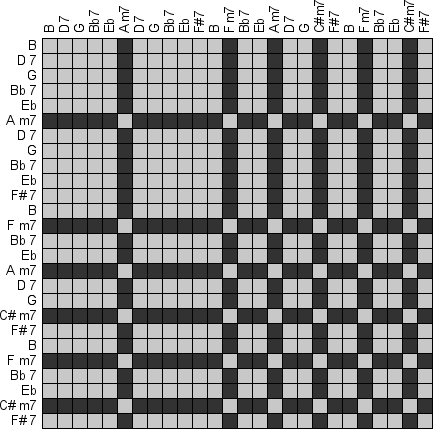
\includegraphics[width=3.5cm]{images/pretty1.jpg}\hspace{0.5cm}
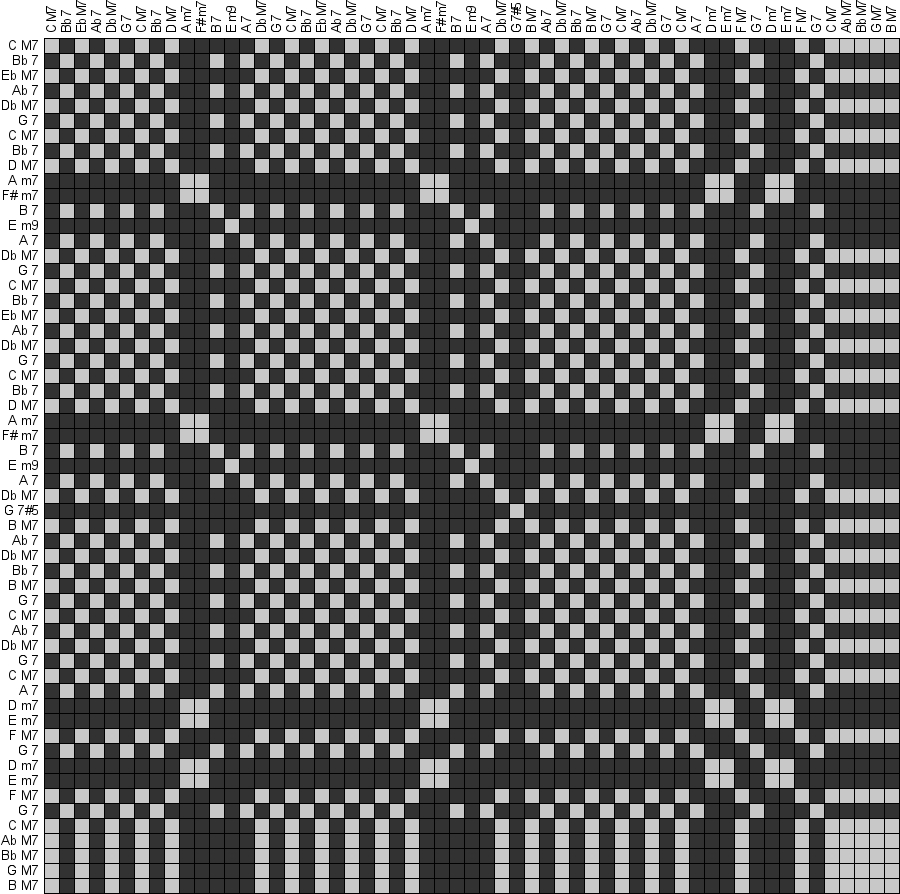
\includegraphics[width=3.5cm]{images/pretty2.jpg}\hspace{0.5cm}
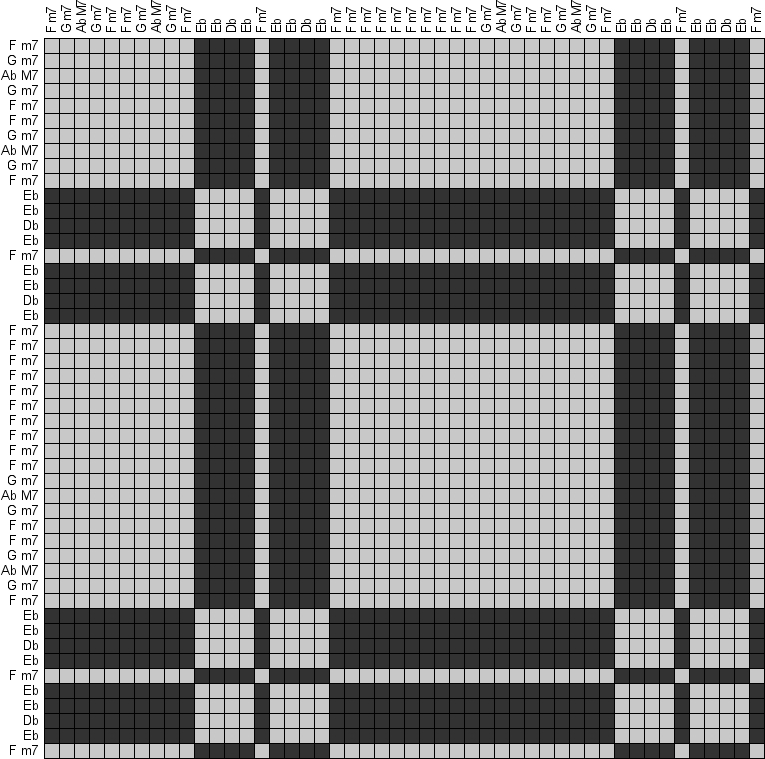
\includegraphics[width=3.5cm]{images/pretty3.jpg}\hspace{0.5cm}
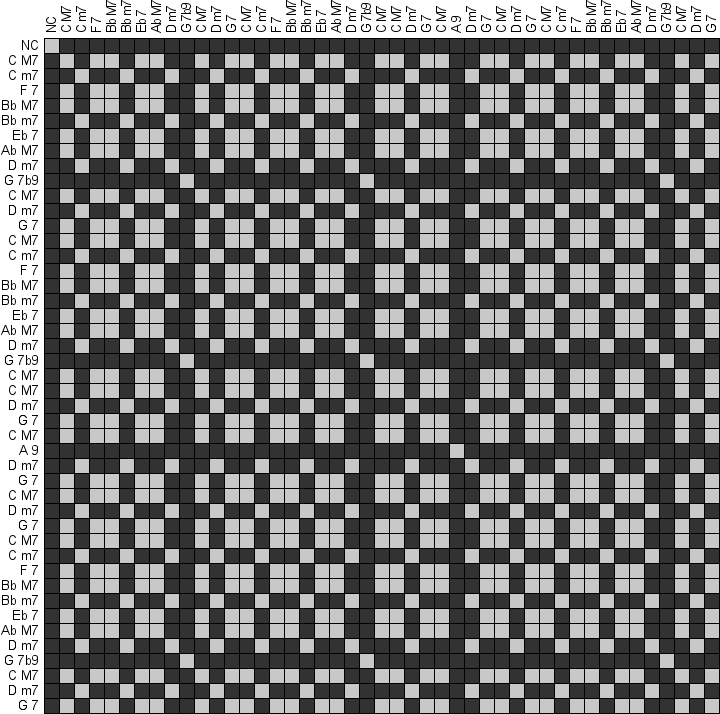
\includegraphics[width=3.5cm]{images/pretty4.jpg}
\caption{Several binary matrices revealing geometrical structure.\label{pretty}}
\end{figure}

My first idea was to compute a segmentation of the piece using the matrix (segmentation is a common way to analyse a music piece, since it gives a global structure). One can often see what looks like a partition of the matrix and consequently of the piece. However, such partitions can appear for different measures, sometimes very different thresholds. They may not appear at all for some pieces, or look very different. So I did not manage to design an algorithm segmenting satisfyingly my data.

The second way that I have been much interested in is \emph{grammatical inference} (or \emph{grammar induction}). As presented in \cite{goldabdallah}, formal grammars, that have been introduced for the modelling of spoken languages, have a lot of applications in computer music. Furthermore, a grammar that could generate a piece or a corpus provides both a synthetic analysis and a way of creating similar pieces.

The problem of grammatical inference is, given two sets $S^+$ and $S^-$ (possibly empty) of words on an alphabet $\Sigma$, to compute a grammar of a certain form (regular grammar, context-free grammar\dots) that generates every word of $S^+$ but none of $S^-$. \cite{bibliogrammar} is a good bibliographical introduction to the topic, and \cite{survey1} and \cite{survey2} a complete survey of state-of-the-art techniques. Several works use grammatical inference on a very close topic to mine: finding a structure inside jazz chords (not like me for a sequence of chords, but for the different chords used in jazz among all the possible combinations of notes) : \cite{jazzgrammar1}, \cite{jazzgrammar2}, \cite{jazzgrammar3}, \cite{jazzgrammar4}.

Nevertheless, I did not find a way of combining my work with these techniques.

In conclusion, I consider that what I did provides an interesting analysis of the data I was given, but that it also reveals potentials still untapped.


\subsection{Improving the compression scheme}

There would be many ways to improve the compression and especially the diagonal compression. Beyond those I already mentioned, I can imagine two important new ones.

The first would be to use information from the melodies as a complement to the chord sequences. There are of course many ways of (and many papers about) combining them. And it would be possible to do so since most of the songs from the database I worked on also contain informations about the melody.

The second would be to incorporate the works described in \cite{aucouturier2002finding}. This papers looks for diagonal patterns (from an audio input), but uses techniques from the field of image analysis (like blurring, convolutions, Hough transform\dots) to identify more sequences as diagonal patterns, even is they are slight holes, or a different orientation (see Figure \ref{aucouturier}). I believe this could improve much the results of the algorithm I used.

\begin{figure}[h!]
\centering
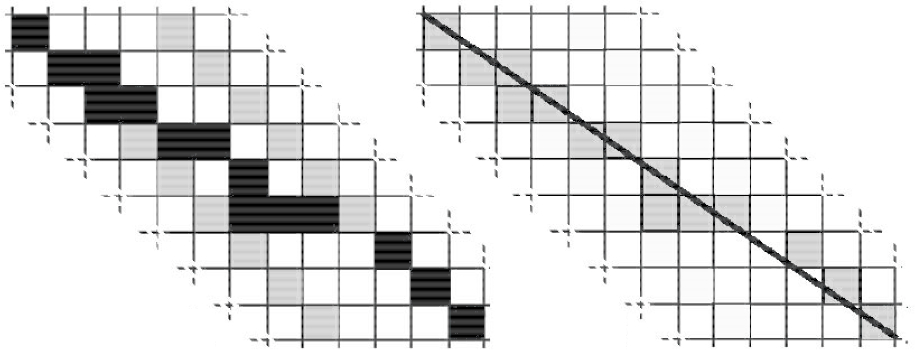
\includegraphics[width=7cm]{images/aucouturier.jpg}
\caption{An \guill{approximate diagonal pattern} (figure from \cite{aucouturier2002finding}).\label{aucouturier}}
\end{figure}

Moreover, since the results on the partial dataset of 30 songs are promising, the algorithms will be tested on the whole corpora, in order to see how the results generalize.


\subsection{The Lrn2Cre8 project}

The Lrn2Cre8 project\footnote{~~\guill{Learn to Create}, see \cite{Lrn2Cre8} for more information.} is a European project between six research institutes working on computer music (Aalborg University being one of them). Its purpose is to develop \emph{learning} techniques of music in order to be able to \emph{create} new pieces. One way consists in adapting to composition already existing analysis methods.

In this context, I discussed with Olivier \textsc{Lartillot}, Ph. D. at Aalborg University, who worked in the same group as I did, about the adaptation of his tool, \textsc{PatMinr} (\cite{patminr}).
While I was trying to use grammatical inference in my own work, it appeared to me that a technique could be combined with his. Described in \cite{bracket2} and used in \cite{bracket1}, it is designed to infer grammar for a specific data, that has been bracketed beforehand so as to emphasize its structure. Originally, this aimed at analysing natural languages, a bracketed data being for instance the sentence \guill{[My neighbour [ate [his yoghurt] [with [a spoon]]]]}.

It made me think of \textsc{PatMinr}, because the resulting decomposition of the melody it performs (Figure \ref{bracket}, on the left) can easily be transformed into a bracketing (Figure \ref{bracket}, on the right; colors are used for visibility but have no meaning). The challenging task, now, is to cleverly label the bracketed piece, before applying the grammar induction methods. This idea is still currently being investigated.

\begin{figure}[h]
\centering
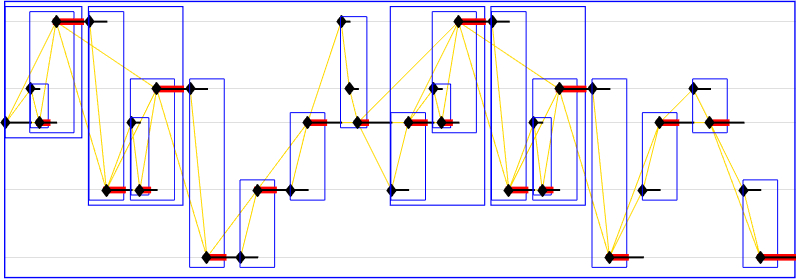
\includegraphics[width=7cm]{images/patminr1.jpg}\hspace{1cm}
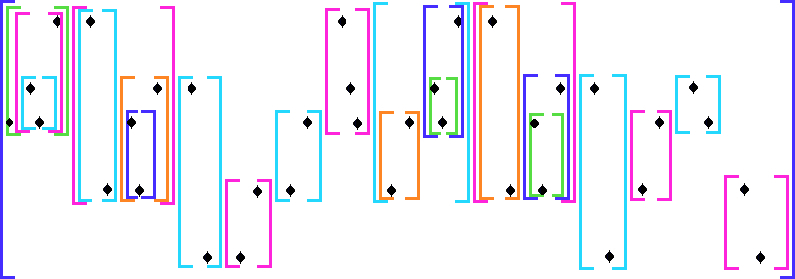
\includegraphics[width=7cm]{images/patminr2.jpg}
\caption{Analysis of a piece with \textsc{PatMinr} and resulting bracketing.\label{bracket}}
\end{figure}


\section{Conclusion}

I have proposed two compression schemes for jazz chord sequences, which perform an interesting analysis of the data I had to study. They combine algorithms for compression without loss and similarity measures loosening the data. The global approach achieves better results than the linear one, showing general structure in jazz.

Moreover, this project brings forward the use of association measures for compression, which can be extended to many others analysis of chords; it asserts the usefulness of the F1-score in this context; and the binary matrices generated with these measures still show important potential for further investigations.

\newpage
%\renewcommand{\baselinestretch}{1}
\section{Bibliography}

\bibliographystyle{plain}
\bibliography{mabiblio}




\end{document}


